% \documentclass[9pt,t]{beamer}
\usefonttheme{professionalfonts}
\usefonttheme{serif}
\PassOptionsToPackage{pdfpagemode=FullScreen}{hyperref}
\PassOptionsToPackage{usenames,dvipsnames}{color}
% \DeclareGraphicsRule{*}{mps}{*}{}
\usepackage{linalgjh}
\usepackage{present}
\usepackage{directories}  % Define \mapdir, \mapmpdir
\usepackage{xr}\externaldocument{\mapdir map1} % read refs from .aux file
\usepackage{catchfilebetweentags}
\usepackage{etoolbox} % from http://tex.stackexchange.com/questions/40699/input-only-part-of-a-file-using-catchfilebetweentags-package
\makeatletter
\patchcmd{\CatchFBT@Fin@l}{\endlinechar\m@ne}{}
  {}{\typeout{Unsuccessful patch!}}
\makeatother

\mode<presentation>
{
  \usetheme{boxes}
  \setbeamercovered{invisible}
  \setbeamertemplate{navigation symbols}{} 
}
\addheadbox{filler}{\ }  % create extra space at top of slide 
\hypersetup{colorlinks=true,linkcolor=blue} 

\title[Isomorphisms] % (optional, use only with long paper titles)
{Three.I Isomorphisms}

\author{\textit{Linear Algebra}, edition four \\ {\small Jim Hef{}feron}}
\institute{
  \texttt{https://hefferon.net/linearalgebra}\\[0.25ex]
  \texttt{http://joshua.smcvt.edu/linearalgebra}
}
\date{}


\subject{Isomorphisms}
% This is only inserted into the PDF information catalog. Can be left
% out. 

\usepackage{cutwin}
\begin{document}
\begin{frame}
  \titlepage
\end{frame}

% =============================================
% \begin{frame}{Reduced Echelon Form} 
% \end{frame}



% ..... Three.I.1 .....
\section{Definition}




%..........
\begin{frame}
\ex
We have the intuition that the vector spaces  
$\Re^2$ and $\polyspace_1$ are ``the same,'' 
in that they are two-component spaces.
For instance 
\begin{align*}
    &\colvec{1 \\ 2}
    \quad\text{is just like}\quad
    1+2x,                            \\
 \text{and}\quad &\colvec{-3 \\ 1/2}
    \quad\text{is just like}\quad
    -3+(1/2)x,                           
\end{align*}
etc.
What makes the spaces alike, not just the sets, is that the association
persists through the operations: this illustrates addition
\begin{multline*}
  \colvec{1 \\ 2}+\colvec{-3 \\ 1/2}=\colvec{-2 \\ 5/2}  \\
  \text{is just like}\quad
  (1+2x)+(-3+(1/2)x)=-2+(5/2)x
\end{multline*}
 and this illustrates scalar multiplication.
\begin{equation*}
  3\colvec{1 \\ 2}=\colvec{3 \\ 6}
  \quad\text{is just like}\quad
  3(1+2x)=3+6x
\end{equation*}
\end{frame}\begin{frame}
\ex
Similarly,
we can link each two-tall vector with a linear polynomial.
\begin{equation*}
  \colvec{a \\ b}
  \quad\longleftrightarrow\quad
  a+bx
\end{equation*}
\pause
This association holds through the vector space operations of
addition
\begin{multline*}
  \colvec{a_1 \\ b_1}+\colvec{a_2 \\ b_2}=\colvec{a_1+a_2 \\ b_1+b_2}    \\
  \quad\longleftrightarrow\quad
  (a_1+b_1x)+(a_2+b_2x)=(a_1+a_2)+(b_1+b_2)x
\end{multline*}
and scalar multiplication.
\begin{equation*}
  r\colvec{a \\ b}=\colvec{ra \\ rb}
  \quad\longleftrightarrow\quad
  r(a+bx)=(ra)+(rb)x
\end{equation*}
We say that the association \definend{preserves the structure} of the spaces.
\end{frame}




%..........
\begin{frame}
\ex
We can think of $\matspace_{\nbyn{2}}$ as ``the same'' as $\Re^4$
if we associate in this way.
\begin{equation*}
  \begin{mat}
    a  &b  \\
    c  &d
  \end{mat}
  \quad\longleftrightarrow\quad
  \colvec{a \\ b \\ c \\ d}
\end{equation*}
For instance, these are corresponding elements.
\begin{equation*}
  \begin{mat}[r]
    1  &-1  \\
    2  &-2
  \end{mat}
  \quad\longleftrightarrow\quad
  \colvec[r]{1 \\ -1 \\ 2 \\ -2}
\end{equation*}
\pause
This association persists under addition.
\begin{multline*}
  \begin{mat}
    a_1  &b_1  \\
    c_1  &d_1
  \end{mat}
  +
  \begin{mat}
    a_2  &b_2  \\
    c_2  &d_2
  \end{mat}
  =
  \begin{mat}
    a_1+a_2  &b_1+b_2  \\
    c_1+c_2  &d_1+d_2
  \end{mat}                                    \\  
  \quad\longleftrightarrow\quad
  \colvec{a_1 \\ b_1 \\ c_1 \\ d_1}
  +
  \colvec{a_2 \\ b_2 \\ c_2 \\ d_2}
  =
  \colvec{a_1+a_2 \\ b_1+b_2 \\ c_1+c_2 \\ d_1+d_2}
\end{multline*}
\end{frame}
\begin{frame}
Here is an example of addition being preserved under this association.
\begin{multline*}
  \begin{mat}
    1  &-1  \\
    2  &-2
  \end{mat}
  +
  \begin{mat}
    0  &4  \\
    3  &-3
  \end{mat}
  =
  \begin{mat}
    1  &3  \\
    5  &-5
  \end{mat}                                    \\  
  \quad\longleftrightarrow\quad
  \colvec{1 \\ -1 \\ 2 \\ -2}
  +
  \colvec{0 \\ 4 \\ 3 \\ -3}
  =
  \colvec{1 \\ 3 \\ 5 \\ -5}
\end{multline*}
\pause
The association also persists through scalar multiplication.
\begin{equation*}
  r\cdot\begin{mat}
   a  &b  \\
   c  &d 
  \end{mat}
  =
  \begin{mat}
    ra  &rb  \\
    rc  &rd
  \end{mat}
  \quad\longleftrightarrow\quad
  r\cdot\colvec{a \\ b \\ c \\ d}
  =
  \colvec{ra \\ rb \\ rc \\ rd} 
\end{equation*}
This illustrates.
\begin{equation*}
  2\cdot\begin{mat}
   1  &-1  \\
   2  &-2 
  \end{mat}
  =
  \begin{mat}
    2  &-2  \\
    4  &-4
  \end{mat}
  \quad\longleftrightarrow\quad
  2\cdot\colvec{1 \\ -1 \\ 2 \\ -1}
  =
  \colvec{2 \\ -2 \\ 4 \\ -4} 
\end{equation*}
\end{frame}




%..........
\begin{frame}{Isomorphism}
\df[def:Isomorphism]
\ExecuteMetaData[\mapdir map1.tex]{df:Isomorphism}
\end{frame}


\begin{frame}{How-to}
To verify that $\map{f}{V}{W}$ is an isomorphism,
do these four.
\begin{itemize}
  \item To show that $f$ is one-to-one, 
    assume that $\vec{v}_1,\vec{v}_2\in V$ are such that
    $f(\vec{v}_1)=f(\vec{v}_2)$
    and derive that $\vec{v}_1=\vec{v}_2$.
  \item To show that $f$ is onto,
    let $\vec{w}$ be an element of $ W$ and find a $\vec{v}\in V$
    such that $f(\vec{v})=\vec{w}$.
  \item To show that $f$ preserves addition, check that for all 
    $\vec{v}_1,\vec{v}_2\in V$
    we have $f(\vec{v}_1+\vec{v}_2)=f(\vec{v}_1)+f(\vec{v}_2)$.
  \item To show that $f$ preserves scalar multiplication, check that for all 
    $\vec{v}\in V$ and $r\in\Re$
    we have $f(r\cdot\vec{v})=r\cdot f(\vec{v})$.
\end{itemize}
The first two cover condition~(1), that the spaces correspond, that 
for each member of~$W$ there exactly one associcated member of~$V$.
The latter two cover~(2), that the map preserves structure.
For these two, the intuition is in the discussion above.
(Later section cover these two at length.)
\end{frame}



%..........
\begin{frame}
\ex
The space of quadratic polynomials $\polyspace_2$ is isomorphic to
$\Re^3$ under this map.
\begin{equation*}
  f(a_0+a_1x+a_2x^2)=\colvec{a_0 \\ a_1 \\ a_2}
\end{equation*}
Here are two examples of the action of $f$.
\begin{equation*}
  f(1+2x+3x^2)=\colvec{1 \\ 2 \\ 3}
  \qquad
  f(3+4x^2)=\colvec{3 \\ 0 \\ 4}  
\end{equation*}
To verify that $f$ is an isomorphism we must check condition~(1), 
that $f$ is a correspondence, and condition~(2), that $f$ preserves structure.
\end{frame}
\begin{frame}
The first part of the definition's clause~(1) is that $f$ is one-to-one.
We suppose $f(\vec{v}_1)=f(\vec{v}_2)$, that the function yields the same output
on two inputs $f(a_0+a_1x+a_2x^2)=f(b_0+b_1x+b_2x^2)$.
From that, we must derive that the two inputs are equal.
The definition of $f$ gives
\begin{equation*}
  \colvec{a_0 \\ a_1 \\ a_2}
  =
  \colvec{b_0 \\ b_1 \\ b_2}
\end{equation*}
and two column vectors are equal only if their entries are equal
$a_0=b_0$, $a_1=b_1$, and~$a_2=b_2$.
Thus the original inputs are equal
$\vec{v}_1=a_0+a_1x+a_2x^2=b_0+b_1x+b_2x^2=\vec{v}_2$.
So $f$ is one-to-one.

\pause
The second part of~(1) is that $f$ is onto.
We consider an element of the codomain
\begin{equation*}
  \vec{w}=\colvec{a_0 \\ a_1 \\ a_2}\in\Re^3
\end{equation*}
and produce an element of the domain that maps to it.
Observe that $\vec{w}$ is the image under $f$ of the member 
$\vec{v}=a_0+a_1x+a_2x^2$ of the domain.
Thus $f$ is onto.
\end{frame}
\begin{frame}
The definition's clause~(2) also has two halves.
First we show that $f$ preserves addition.
Consider $f$ acting on the sum of two elements of the domain.
\begin{multline*}
  f(\,(a_0+a_1x+a_2x^2)+(b_0+b_1x+b_2x^2)\,)  \\
  =f(\,(a_0+b_0)+(a_1+b_1)x+(a_2+b_2)x^2\,)
\end{multline*}
The definition of $f$ gives
\begin{equation*}
  =\colvec{a_0+b_0 \\ a_1+b_1 \\ a_2+b_2}
\end{equation*}
and that equals
\begin{equation*}
  =\colvec{a_0 \\ a_1 \\ a_2}
  +
  \colvec{b_0 \\ b_1 \\ b_2}
\end{equation*}
which gives
\begin{equation*}
  =f(\,a_0+a_1x+a_2x^2)+f(b_0+b_1x+b_2x^2\,)
\end{equation*}
as required.
\end{frame}
\begin{frame}
We finish by checking that $f$ preserves scalar multiplication.
This is similar to the check for addition.
\begin{align*}
  f(r\cdot(a_0+a_1x+a_2x^2))
  &=f(\,(ra_0)+(ra_1)x+(ra_2)x^2\,) \\
   &=\colvec{ra_0 \\ ra_1 \\ ra_2}  \\ 
   &=r\cdot\colvec{a_0 \\ a_1 \\ a_2}   \\ 
   &=r\cdot f(\,a_0+a_1x+a_2x^2\,)
\end{align*}

\pause
\bigskip
So the function~$f$ is an isomorphism.
Because there is an isomorphism, the two spaces are isomorphic
$\polyspace_2\isomorphicto \Re^3$. 
% \qed
\end{frame}



\begin{frame}
\ex Consider these two vector spaces (under the natural operations)
\begin{equation*}
  V=\set{
    \begin{mat}
      a &b \\
      c &0
    \end{mat}
    \suchthat a,b,c\in\Re}
  \qquad
  W=\set{\rowvec{x &y &z}\suchthat x,y,z\in\Re}
\end{equation*}
and consider this function.
\begin{equation*}
  \begin{mat}
    a &b \\
    c &0
  \end{mat}
  \mapsunder{f}
  \rowvec{b &2a &a+c}
\end{equation*}
Here is an example of the map's action.
\begin{equation*}
  \begin{mat}
    3 &2 \\
    1 &0
  \end{mat}
  \mapsunder{f}
  \rowvec{2 &6 &4}
\end{equation*}
We will verify that $f$
is an isomorphism.
\end{frame}
\begin{frame}
To show that $f$ is one-to-one, suppose that
\begin{equation*}
  f(\begin{mat}
    a_1 &b_1 \\
    c_1 &0
  \end{mat})
  =
  f(\begin{mat}
    a_2 &b_2 \\
    c_2 &0
  \end{mat})
\end{equation*}
Then $\rowvec{b_1 &2a_1 &a_1+c_1}=\rowvec{b_2 &2a_2 &a_2+c_2}$.
The first entries give that $b_1=b_2$, the second entries that $a_1=a_2$, 
and with that the third entries give that $c_1=c_2$.
\begin{equation*}
  \begin{mat}
    a_1 &b_1 \\
    c_1 &0
  \end{mat}
  =
  \begin{mat}
    a_2 &b_2 \\
    c_2 &0
  \end{mat}
\end{equation*}

\pause
To show that $f$ is onto, consider a member of $W$.
\begin{equation*}
  \vec{w}=\rowvec{x &y &z}
\end{equation*}
We must find a $\vec{v}$ so that $f(\vec{v})=\vec{w}$.
The map sends the upper right entry of the input to
the first entry of the output, so the upper right of~$\vec{v}$ 
is~$x$.
Similarly, the upper left of~$\vec{v}$ is $(1/2)y$.
With that, the lower left is $z-(1/2)y$.
\begin{equation*}
  \rowvec{x &y &z}
  =f(\begin{mat}
    y/2    &x \\
    z-y/2  &0
  \end{mat})
\end{equation*}
\end{frame}
\begin{frame}
To show that $f$ preserves addition, assume
\begin{equation*}
 f(
  \begin{mat}
    a_1 &b_1 \\
    c_1 &0
  \end{mat}
  +
  \begin{mat}
    a_2 &b_2 \\
    c_2 &0
  \end{mat}
  )
  =f(
  \begin{mat}
    a_1+a_2 &b_1+b_2 \\
    c_1+c_2 &0
  \end{mat}
  )
\end{equation*}
which equals $\rowvec{b_1+b_2 &2(a_1+a_2) &(a_1+a_2)+(c_1+c_2)}$.
In turn, that equals this. 
\begin{equation*}
\rowvec{b_1 &2a_1 &a_1+c_1}+\rowvec{b_2 &2a_2 &a_2+c_2}
  =f(
  \begin{mat}
    a_1 &b_1 \\
    c_1 &0
  \end{mat})
  +
  f(
  \begin{mat}
    a_2 &b_2 \\
    c_2 &0
  \end{mat})
\end{equation*}

\pause
Preservation of scalar multiplication is similar.
\begin{align*}
  f(r\cdot
  \begin{mat}
    a &b \\
    c &0
  \end{mat}
  )
  &=f(
  \begin{mat}
    ra &rb \\
    rc &0
  \end{mat}
  )                                 \\
  &=\rowvec{rb &2ra &ra+rc}         \\
  &=r\cdot\rowvec{b &2a &a+c}         \\
  &=r\cdot f(
  \begin{mat}
    a &b \\
    c &0
  \end{mat}
  )
\end{align*}
\end{frame}





%..........
\begin{frame}{Preservation is special}
Many functions do not preserve addition and scalar multiplication.
For instance, $\map{f}{\Re^2}{\Re^2}$
\begin{equation*}
  f(\colvec{x \\ y})=\colvec{x^2 \\ y^2}
\end{equation*}
does not preserve addition since the sum done one way 
\begin{equation*}
  f(\colvec{1 \\ 0}+\colvec{2 \\ 0})=f(\colvec{3 \\ 0})=\colvec{9 \\ 0}
\end{equation*}
gives a different result than the sum done the other way.
\begin{equation*}
  f(\colvec{1 \\ 0})+f(\colvec{2 \\ 0})=\colvec{1 \\ 0}+\colvec{4 \\ 0}
  =\colvec{5 \\ 0}
\end{equation*}
\end{frame}


%..........
\begin{frame}{Special case: Automorphisms}
\df[df:Automorphism]\hspace*{-1em}
\ExecuteMetaData[\mapdir map1.tex]{df:Automorphism}

\pause
\ex[exam:RigidPlaneMapsAutos]\hspace*{-1em}
\ExecuteMetaData[\mapdir map1.tex]{ex:RigidPlaneMapsAutos0}
\centergraphic{\mapmpdir ch3.14}

\pause
\ExecuteMetaData[\mapdir map1.tex]{ex:RigidPlaneMapsAutos1}
\centergraphic{\mapmpdir ch3.15}
\end{frame}
\begin{frame}
\ExecuteMetaData[\mapdir map1.tex]{ex:RigidPlaneMapsAutos2}
\centergraphic{\mapmpdir ch3.16}
Checking that each is an isomorphism is an exercise.

\bigskip
\pause
Why study automorphisms?
Isn't it trivial that the plane is just like itself?

Consider the family of automorphisms~$t_{\Theta}$ 
rotating all vectors counterclockwise.
They makes precise the intuition that
the plane is uniform\Dash that space near the $x$-axis
is just like space near the $y$-axis. 
\end{frame}
\begin{frame}
So one lesson is that we can use maps
to describe relationships between spaces. 
If the maps are isomorphisms then this relation
makes precise the intuition ``just like''. 

A second lesson is that while there is an obvious automorphism
of~$\Re^2$
\begin{equation*}
  \colvec{x \\ y}\mapsto\colvec{x \\ y}
\end{equation*}
there are reasons to consider maps other than
the obvious one.
\end{frame}



%..........
\begin{frame}
\lm[le:IsoSendsZeroToZero]
\ExecuteMetaData[\mapdir map1.tex]{lm:IsoSendsZeroToZero}

\pause
\pf
\ExecuteMetaData[\mapdir map1.tex]{pf:IsoSendsZeroToZero}
\qed
\end{frame}




%..........
\begin{frame}
\lm[le:PresStructIffPresCombos]
\ExecuteMetaData[\mapdir map1.tex]{lm:PresStructIffPresCombos}

\iftoggle{showallproofs}{
  \pause
  \pf
  \ExecuteMetaData[\mapdir map1.tex]{pf:PresStructIffPresCombos0}

  \pause
  \ExecuteMetaData[\mapdir map1.tex]{pf:PresStructIffPresCombos1}
}{

  \medskip
  The book contains the details of both proofs.

  \medskip\re
  Examination of the proofs show that they depend only on 
  clause~(2) of the definition, not on that the map is a 
  correspondence.
  We will say more in the next section.
}
\end{frame}
\iftoggle{showallproofs}{
  \begin{frame}
  \ExecuteMetaData[\mapdir map1.tex]{pf:PresStructIffPresCombos2}
  \qed
  \end{frame}
}{}


%..........
\begin{frame}
% This result eases checking that a function preserves
% the structure of a vector space, since we can do it in one step
% with statement~(2).   

\ex
The line through the origin with slope two
is a vector space.
% \begin{graphicbytext}{0.15}{asy/three_i_line.pdf}
\begin{center}
  $L=\set{\colvec{x \\ y}\suchthat y=2x}
   =\set{\colvec{t \\ 2t}\suchthat t\in\Re}$
  \qquad
  \vcenteredhbox{\includegraphics{asy/three_i_line.pdf}}
\end{center}
% \end{graphicbytext}
The parametrization
\begin{equation*}
  L=\set{\colvec{t \\ 2t}\suchthat t\in\Re}
   =\set{t\cdot\colvec{1 \\ 2} \suchthat t\in\Re}
\end{equation*}
suggests that $L$ is just like~$\Re$:
there is a point on~$L$
% \begin{equation*}
%   1\cdot\colvec{1 \\ 2}
% \end{equation*}
associated with $1\in\Re$,
a point associated with $2\in\Re$, etc.
We will show that this function is an isomorphism between $L$
and~$\Re^1$.
\begin{equation*}
  f(\,\colvec{t \\ 2t}\,)
  =t
\end{equation*}
\end{frame}
\begin{frame}
To verify that $f$ is one-to-one
suppose that $f$ maps two members of $L$ to the same output.
\begin{equation*}
  f(\,t_1\cdot\colvec{1 \\ 2}\,)=f(\,t_2\cdot\colvec{1 \\ 2}\,)
\end{equation*}
By the definition of~$f$ we have $t_1=t_2$ and so the two
input members of $L$ are equal.

To check that $f$ is onto
consider a member of the codomain, $r\in\Re$.
There is a member of the domain~$L$ that maps to it, namely this one.
\begin{equation*}
  f(\,r\cdot\colvec{1 \\ 2}\,)=r
\end{equation*}
% Thus $f$ is onto.

To finish, we combine the two structure checks,  using the lemma's~(2).
\begin{multline*}
  f(\,c_1\cdot\colvec{t_1 \\ 2t_1}+c_2\cdot\colvec{t_2 \\ 2t_2}\,)
  =f(\,(c_1t_1+c_2t_2)\cdot\colvec{1 \\ 2}\,)                    \\
  =c_1t_1+c_2t_2   
  =
  c_1\cdot f(\,\colvec{t_1 \\ 2t_1}\,)+c_2\cdot f(\,\colvec{t_2 \\ 2t_2}\,)
\end{multline*}

\end{frame}



% ..... Three.I.2 .....
\section{Dimension characterizes isomorphism}
%..........
\begin{frame}
\lm[lem:IsoInvAlsoIso]
\ExecuteMetaData[\mapdir map1.tex]{lm:IsoInvAlsoIso}

\pause
\pf
\ExecuteMetaData[\mapdir map1.tex]{pf:IsoInvAlsoIso0}

\pause
\ExecuteMetaData[\mapdir map1.tex]{pf:IsoInvAlsoIso1}
\qed
\end{frame}


\begin{frame}
% \begin{graphicbytext}{0.1}{asy/three_i_line.pdf}
\ex
We saw earlier that
this line through the origin subspace of~$\Re^2$
\begin{equation*}
  L=\set{\colvec{t \\ 2t} \suchthat t\in\Re}
\end{equation*}
% \end{graphicbytext}
\noindent is isomorphic to $\Re^1$
via this function.
\begin{equation*}
  f(\,t\cdot\colvec{1 \\ 2}\,)=t
\end{equation*}  
The inverse $\map{f^{-1}}{\Re}{L}$ 
given by
\begin{equation*}
  f^{-1}(r)=r\cdot\colvec{1 \\ 2}=\colvec{r \\ 2r}
\end{equation*}
is also an isomorphism.
\end{frame}



%..........
\begin{frame}
\th[th:IsoEquivRel]
\ExecuteMetaData[\mapdir map1.tex]{th:IsoEquivRel}

\iftoggle{showallproofs}{
  \pause
  \pf
  \ExecuteMetaData[\mapdir map1.tex]{pf:IsoEquivRel0}
  
  \pause
  \ExecuteMetaData[\mapdir map1.tex]{pf:IsoEquivRel1}
}{
  \medskip
  The book contains the proof; here is a diagram of what it
  tells us:
  the collection of all finite-dimensional vector spaces
  is partitioned into classes.
  Two spaces are in the same class if they are isomorphic.
  \centergraphic{\mapmpdir ch3.17}
  The next result characterizes these classes.
}
\end{frame}
\iftoggle{showallproofs}{
  \begin{frame}
  \ExecuteMetaData[\mapdir map1.tex]{pf:IsoEquivRel2}
  \qed

  So
  the collection of spaces
  is partitioned into classes with
  two spaces in the same class if and only if they are isomorphic.
  \centergraphic{\mapmpdir ch3.17}
  \end{frame}
}{
}




%..........
\begin{frame}
\th[th:NDimSpaceIsoRN]
\ExecuteMetaData[\mapdir map1.tex]{th:NDimSpaceIsoRN}

\medskip
The proof is these two lemmas.
\medskip

\pause
\lm[lem:IsoImpliesSameDim]
\ExecuteMetaData[\mapdir map1.tex]{lm:IsoImpliesSameDim}

\lm[lem:EqDimImpIso]
\ExecuteMetaData[\mapdir map1.tex]{lm:EqDimImpIso}

\iftoggle{showallproofs}{
   \medskip\par
   We prove them separately below.
}{
    \medskip\par
    The proof of the first depends on showing that 
    under a isomorphism the image of a domain basis 
    is a range basis.
    The proof of the second depends on giving an explicit 
    isomorphism from an $n$-dimensional domain to $\Re^n$.    
    See the book for the full proofs; 
    here we will illustrate with an example.
}
\end{frame}


%..........
\iftoggle{showallproofs}{
  \begin{frame}
  \lm[lem:IsoImpliesSameDim]
  \ExecuteMetaData[\mapdir map1.tex]{lm:IsoImpliesSameDim}

  \pf
  \ExecuteMetaData[\mapdir map1.tex]{pf:IsoImpliesSameDim0}
  \end{frame}
  \begin{frame}
  \ExecuteMetaData[\mapdir map1.tex]{pf:IsoImpliesSameDim1}
  \qed
  \end{frame}

  %..........
  \begin{frame}
  \lm[lem:EqDimImpIso]
  \ExecuteMetaData[\mapdir map1.tex]{lm:EqDimImpIso}

  \pause
  \pf
  \ExecuteMetaData[\mapdir map1.tex]{pf:EqDimImpIso0}

  \pause
  \ExecuteMetaData[\mapdir map1.tex]{pf:EqDimImpIso1}
  \end{frame}
  \begin{frame}
  \ExecuteMetaData[\mapdir map1.tex]{pf:EqDimImpIso2}

  \pause
  \ExecuteMetaData[\mapdir map1.tex]{pf:EqDimImpIso3}
  \end{frame}
  \begin{frame}
  \ExecuteMetaData[\mapdir map1.tex]{pf:EqDimImpIso4}
  \qed

  \pause
  \medskip
  \no
  The second paragraph's 
  representation map $\text{Rep}_B$ is a well-defined function since
  for each basis,
  every vector $\vec{v}$ has a unique representation with respect to that basis.
  \end{frame}
}{}

\begin{frame}
\ex
The plane $2x-y+z=0$ through the origin in $\Re^3$ is a vector space
(under the natural operations).
\begin{center}
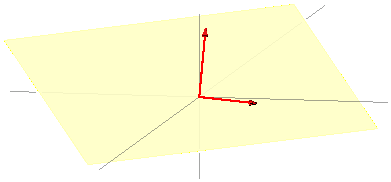
\includegraphics[scale=.8]{asy/three_i_plane.pdf}
\end{center}
  Describe the space as a span by taking that to be a one-equation 
  linear system
  and parametrizing $x=(1/2)y-(1/2)z$.
  \begin{equation*}
    P=\set{\colvec{1/2 \\ 1 \\ 0}y
            +\colvec{-1/2 \\ 0 \\ 1}z
           \suchthat y,z\in\Re}
  \end{equation*}
  Clearly the set with those two vectors is linearly independent so it is
  a basis.
\begin{equation*}
  B=\sequence{\colvec{1/2 \\ 1 \\ 0},
              \colvec{-1/2 \\ 0 \\ 1}}
\end{equation*}
\end{frame}

\begin{frame}\vspace*{-2ex}
% \begin{graphicbytextright}{0.3}{asy/three_i_plane.pdf}
Here is the basis from the prior slide.
\begin{equation*}
  B=\sequence{\colvec{1/2 \\ 1 \\ 0},
              \colvec{-1/2 \\ 0 \\ 1}}
\end{equation*}
Because its basis has two vectors, $P$ is a dimension~$2$ space. 
% \end{graphicbytextright}

  The second lemma's proof
  shows that this is an isomorphism: the map $\map{f}{P}{\Re^2}$ that 
  associates each element~$\vec{v}\in P$
  with its representation $\rep{\vec{v}}{B}\in\Re^2$.

  To illustrate the association, 
  here is an example of its action on an $\Re^2$ vector picked at random.
  \begin{equation*}
    \vec{v}_1=\colvec{7/2 \\ 3 \\ -4}=\colvec{1/2 \\ 1 \\ 0}\cdot 3
           +\colvec{-1/2 \\ 0 \\ 1}\cdot (-4)
    \quad\mapsunder{f}\quad
    \rep{\vec{v}_1}{B}=\colvec{3 \\ -4}
  \end{equation*}
  \pause
  Another (as with the prior one, $\vec{v}_2$ is picked at random from $\Re^2$).
  \begin{equation*}
    \vec{v}_2=\colvec{-17/4 \\ 1/2 \\ 9}=\colvec{1/2 \\ 1 \\ 0}\cdot (1/2)
           +\colvec{-1/2 \\ 0 \\ 1}\cdot 9
    \quad\mapsunder{f}\quad
    \rep{\vec{v}_2}{B}=\colvec{1/2 \\ 9}
  \end{equation*}
\end{frame}
\begin{frame}
  The first lemma's proof shows that any isomorphism takes bases to bases:
  starting with  basis vectors
  $\vec{\beta}_i$ for the domain and applying an isomorphism~$f$ gives
  basis vectors $f(\vec{\beta}_i)$ for the range.

  For the isomorphism from the prior slide we have
  \begin{equation*}
    \vec{\beta}_1=\colvec{1/2 \\ 1 \\ 0}\cdot 1
           +\colvec{-1/2 \\ 0 \\ 1}\cdot 0
    \quad\mapsunder{f}\quad
    \colvec{1 \\ 0}
  \end{equation*}
  and
  \begin{equation*}
    \vec{\beta}_2=\colvec{1/2 \\ 1 \\ 0}\cdot 0
           +\colvec{-1/2 \\ 0 \\ 1}\cdot 1
    \quad\mapsunder{f}\quad
    \colvec{0 \\ 1}
  \end{equation*}
  which together make the basis $\stdbasis_2$ for $\Re^2$.
\end{frame}








%..........
\begin{frame}
\co[co:FiniteDimensionalIsoToReN]
\ExecuteMetaData[\mapdir map1.tex]{co:FiniteDimensionalIsoToReN}

\pause
\medskip
Thus the real spaces $\Re^n$ form a set of canonical
representatives of the isomorphism classes\Dash every 
isomorphism class contains one and only one~$\Re^n$.
\centergraphic{\mapmpdir ch3.18}
\end{frame}



%...........................
% \begin{frame}
% \ExecuteMetaData[../gr3.tex]{GaussJordanReduction}
% \df[def:RedEchForm]
% 
% \end{frame}
\end{document}
